\section{网络科学基础理论}
%本章主要介绍了网络科学的一些基本概念,梳理了复杂网络常用的算法模型。
\subsection{复杂网络概述}
复杂网络由节点和节点之间的连边构成,对真实系统中各种各样的复杂关系有着统一的描述方式。
例如在社交关系中,社交个体作为节点,个体与个体之间的社交关系作为连边,由此构成了社交网络。
除了描述各种真实系统外,复杂网络也涌现出了诸如自组织、自相似性、小世界现象、社团集群等多种有趣的性质 \cite{Strogatz2001}。

\subsubsection{复杂网络的拓扑结构}
复杂网络$ G = (V, E) $通常由$ N=|V| $个节点和$ |E| $条连边构成。
其中,$ V $是网络$ G $的节点集合,$ E $是网络$ G $的边集合。
通常来说,通过节点的边是否有向、是否有权重可将复杂网络划分为$ 4 $种类型:
(1)无向无权重网络,(2)无向有权重网络,(3)有向无权重网络,(4)有向有权重网络。
以城市道路网络为例,将不同的城市定义为网络的节点,城市之间是否可以直达作为连边,就得到了原始的无向无权重网络。
不同城市之间存在距离的远近,将这种距离关系映射到城市道路网络中时,就得到了无向有权重网络。
考虑到有些城市之间的交通可能只存在单向行车道,将这种关系映射到城市道路网络中,就得到了有向无权重网络。
同样,将以上两个因素都考虑到,就得到了有向有权重网络。

\begin{figure}[ht]
	\centering
	\subfigure[无向无权重网络]{
		\label{2DSF_1} %% label for first subfigure
		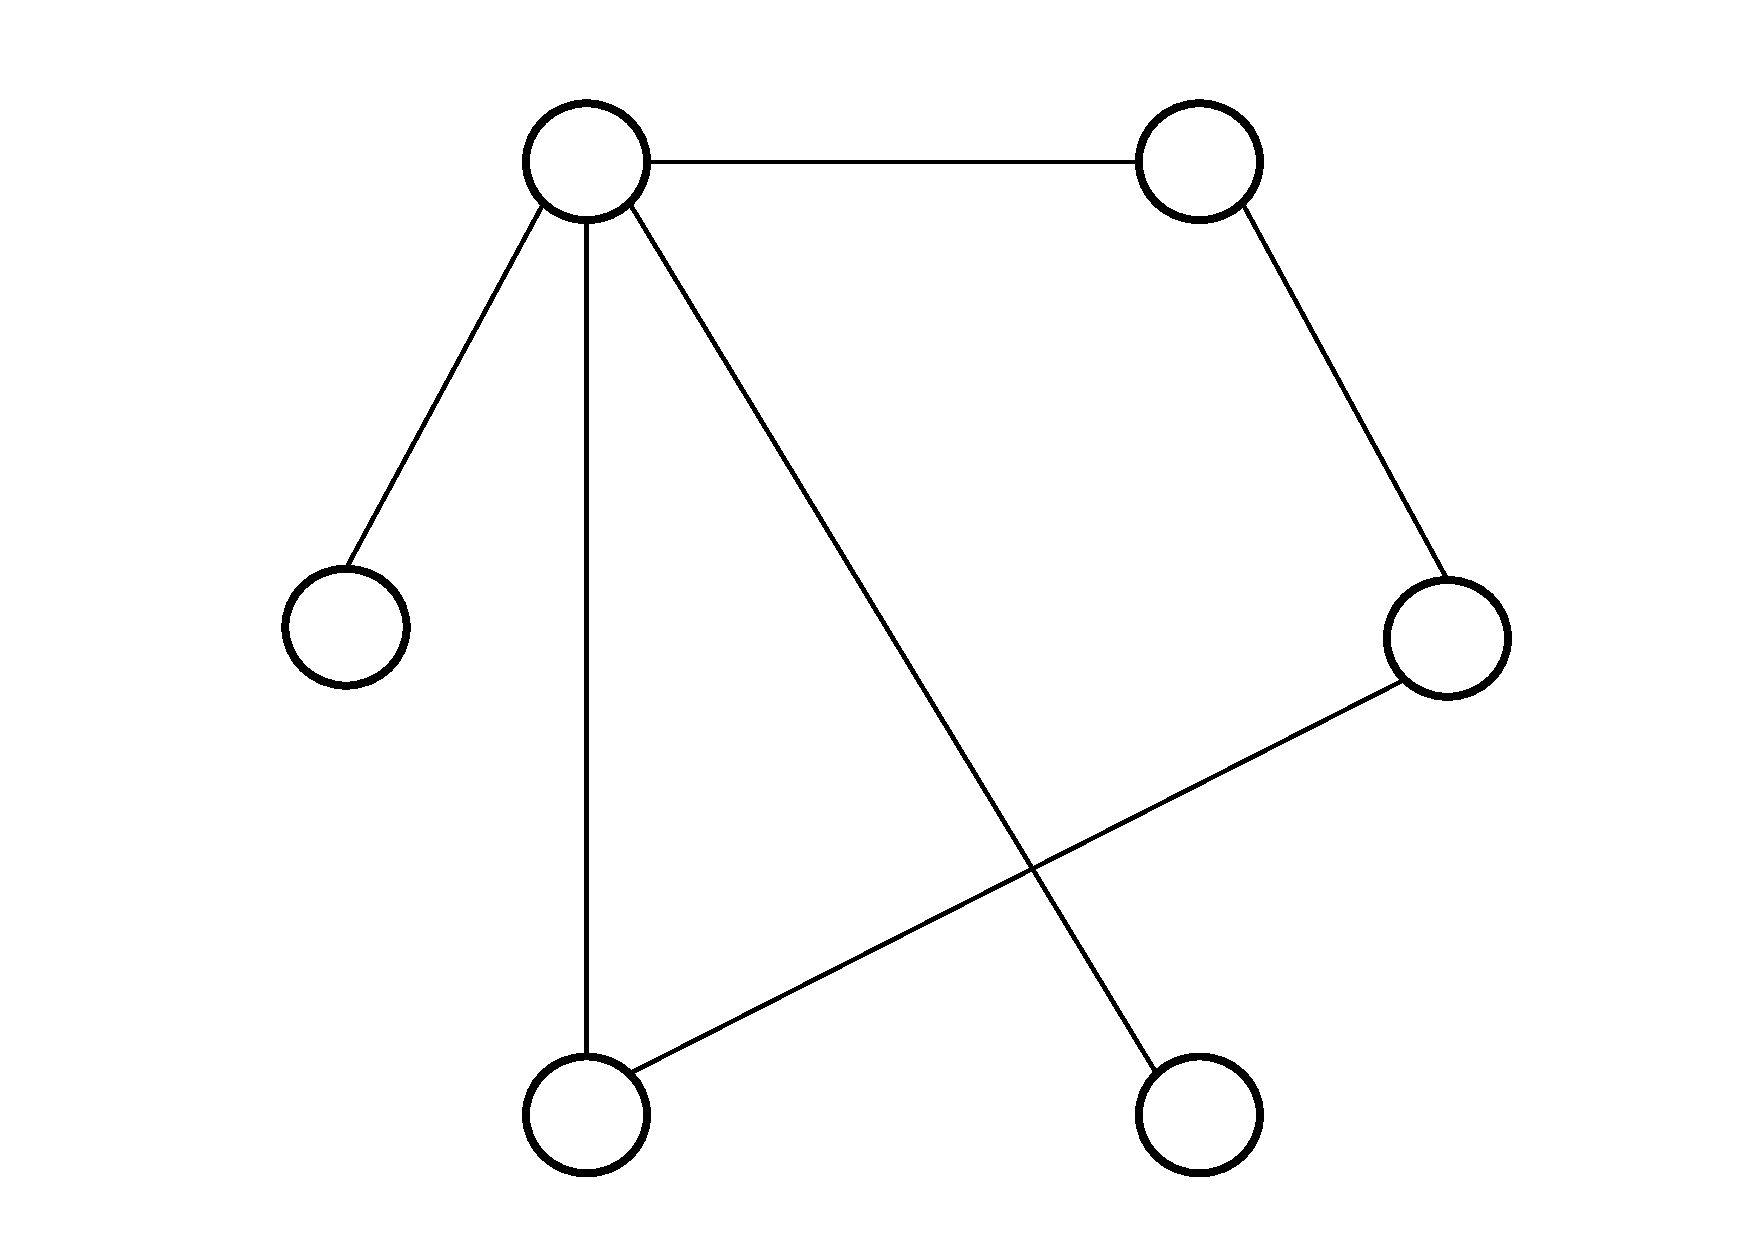
\includegraphics[width=0.3\columnwidth]{chapter2Fig/无向无权重.pdf}}\hfil
	\subfigure[无向有权重网络]{
		\label{2DSF_2} %% label for second subfigure
		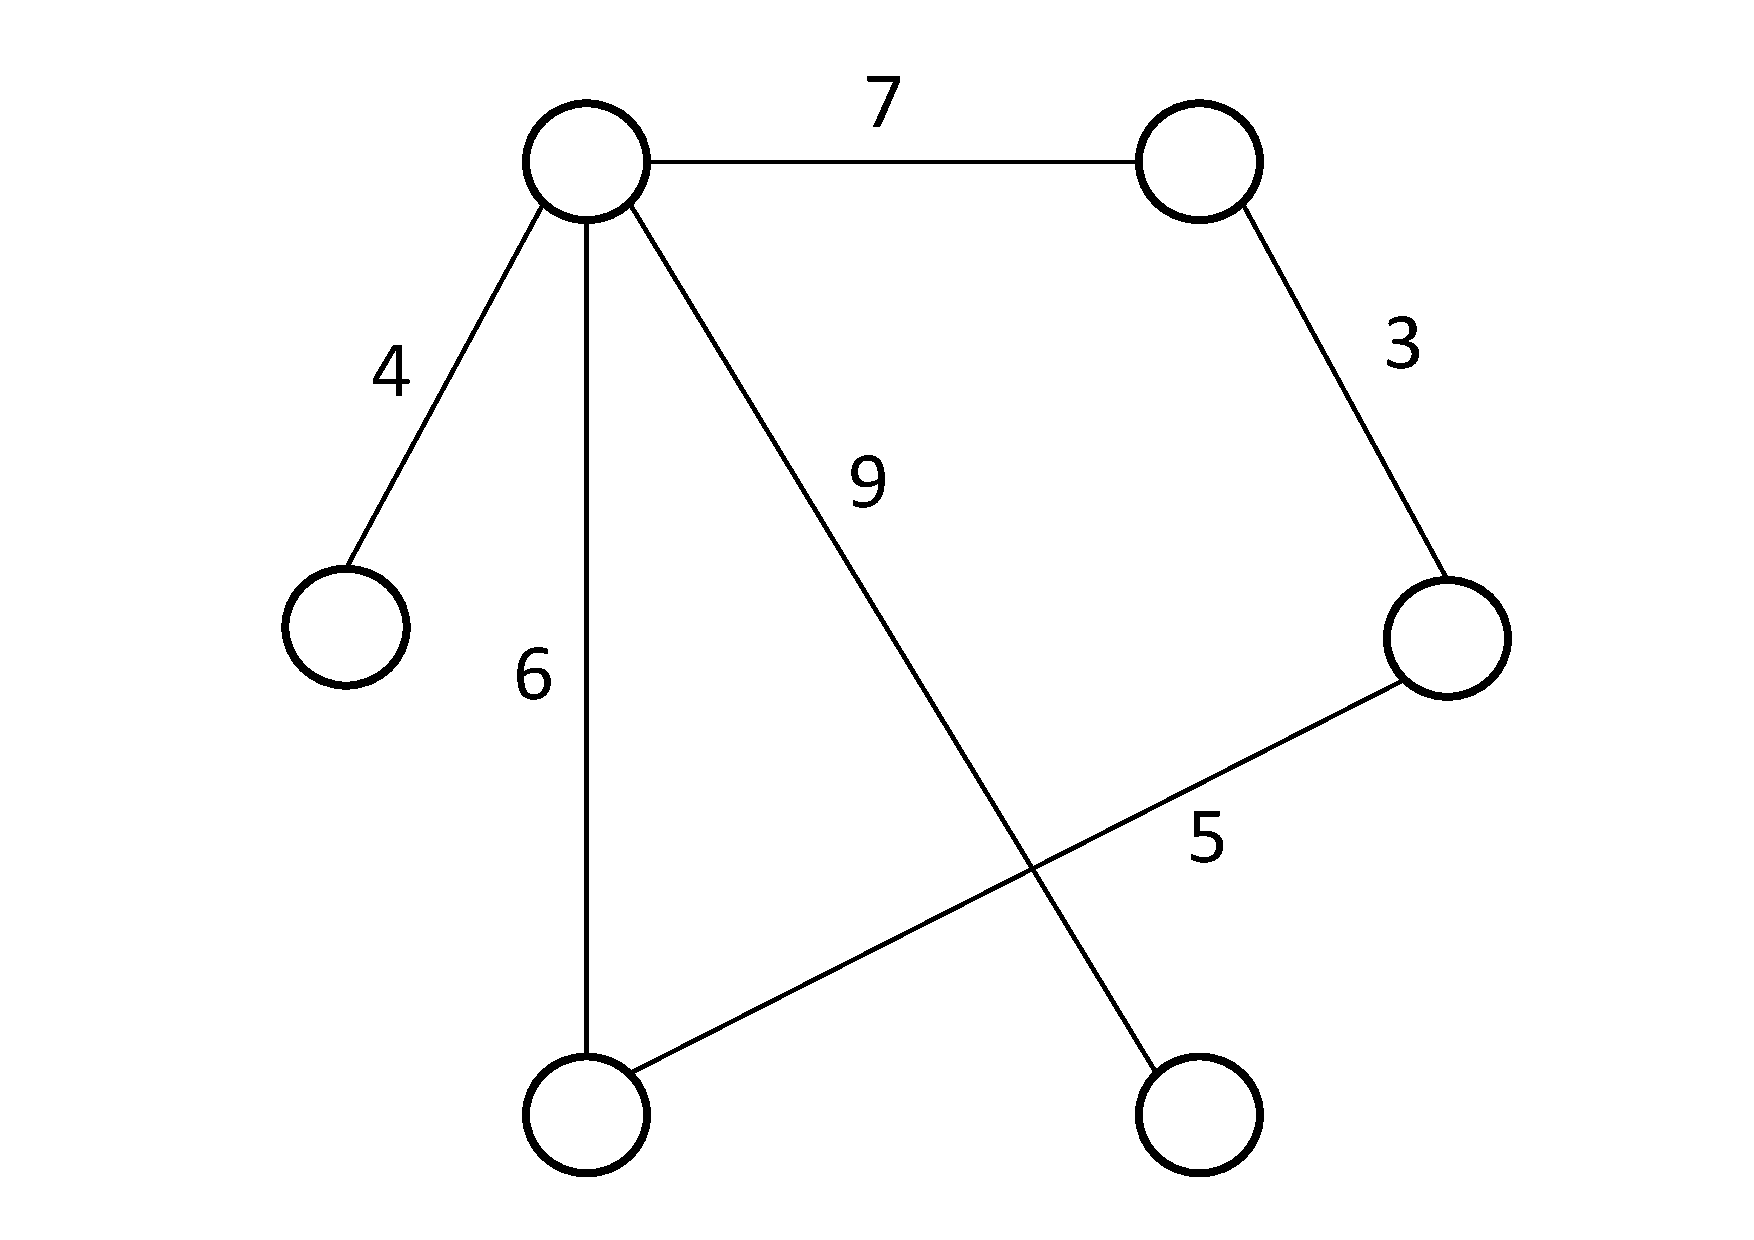
\includegraphics[width=0.3\columnwidth]{chapter2Fig/无向有权重.pdf}}
	
	\subfigure[有向无权重网络]{
		\label{2DSF_3} %% label for first subfigure
		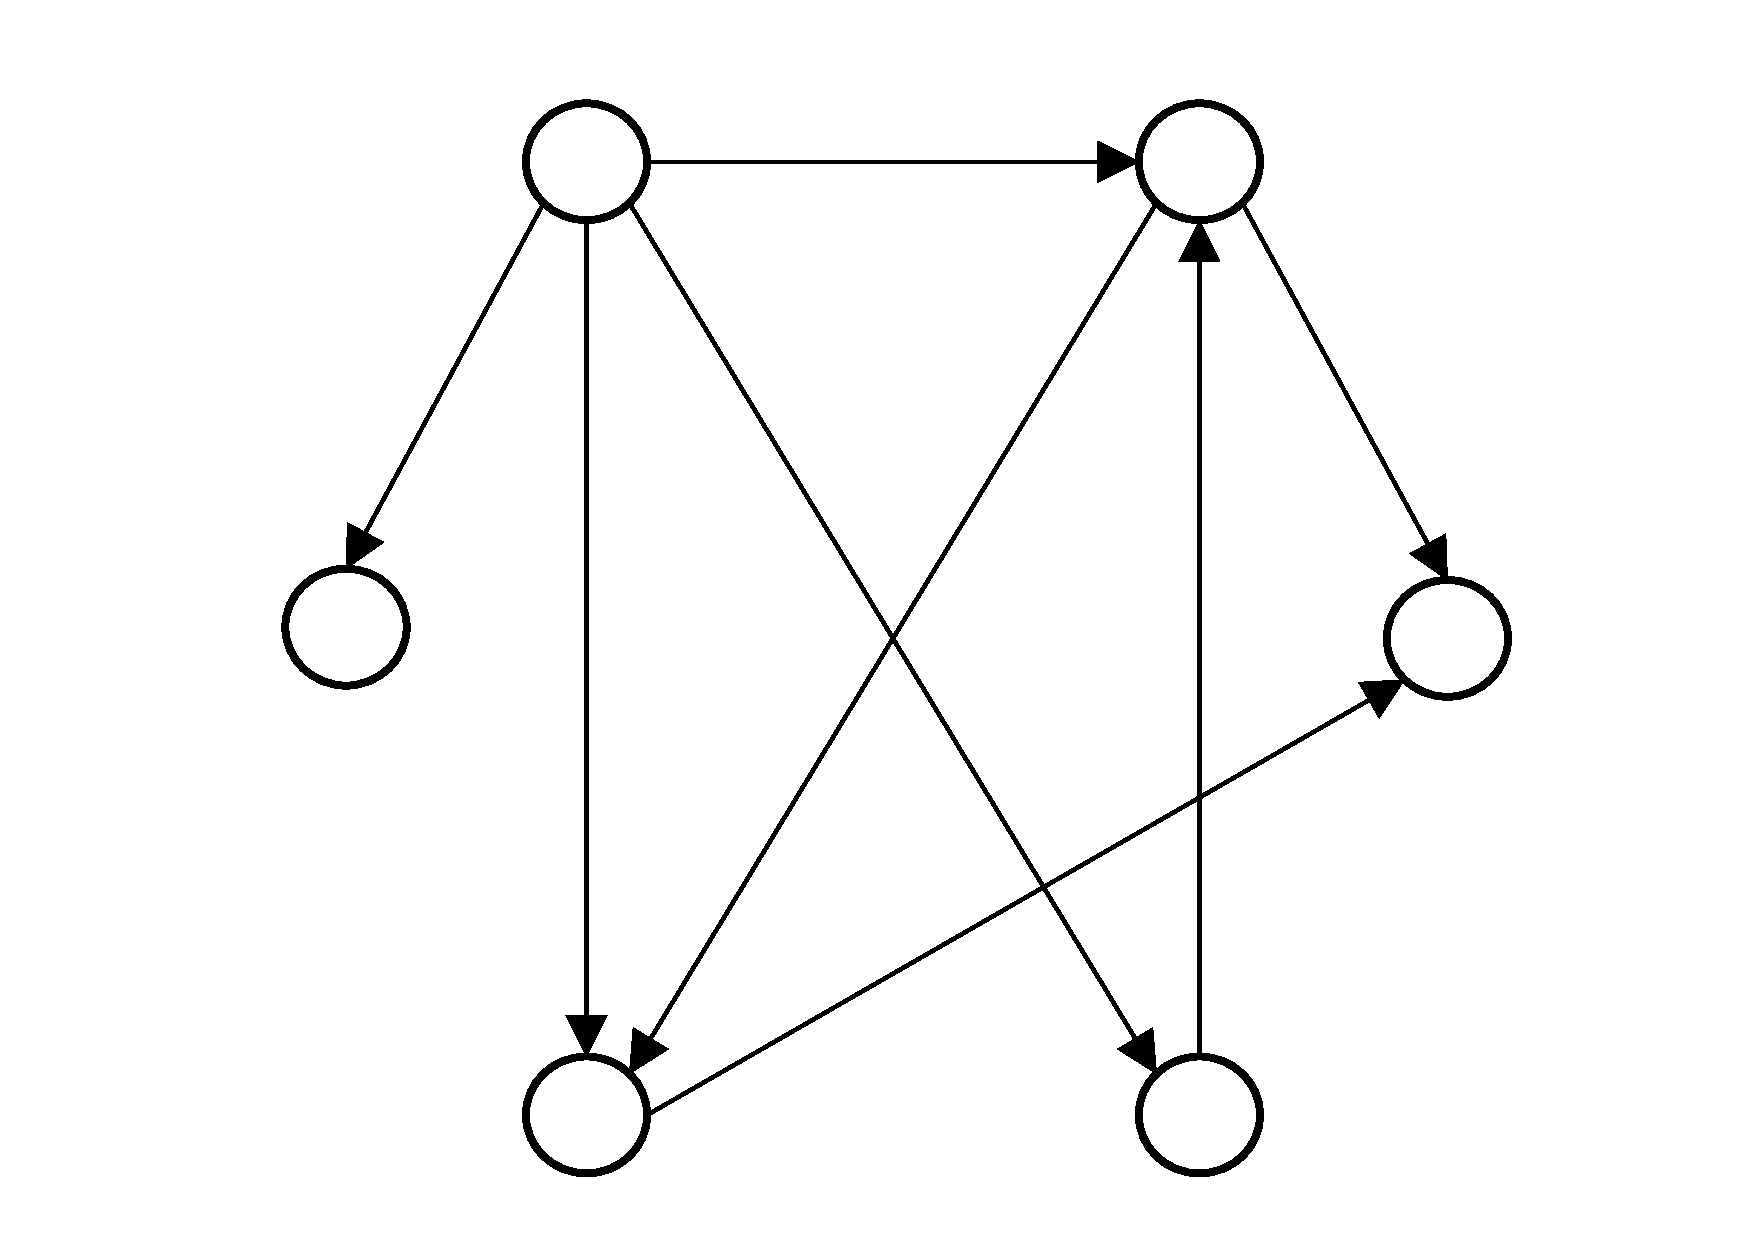
\includegraphics[width=0.3\columnwidth]{chapter2Fig/有向无权重.pdf}}\hfil
	\subfigure[有向有权重网络]{
		\label{2DSF_4} %% label for first subfigure
		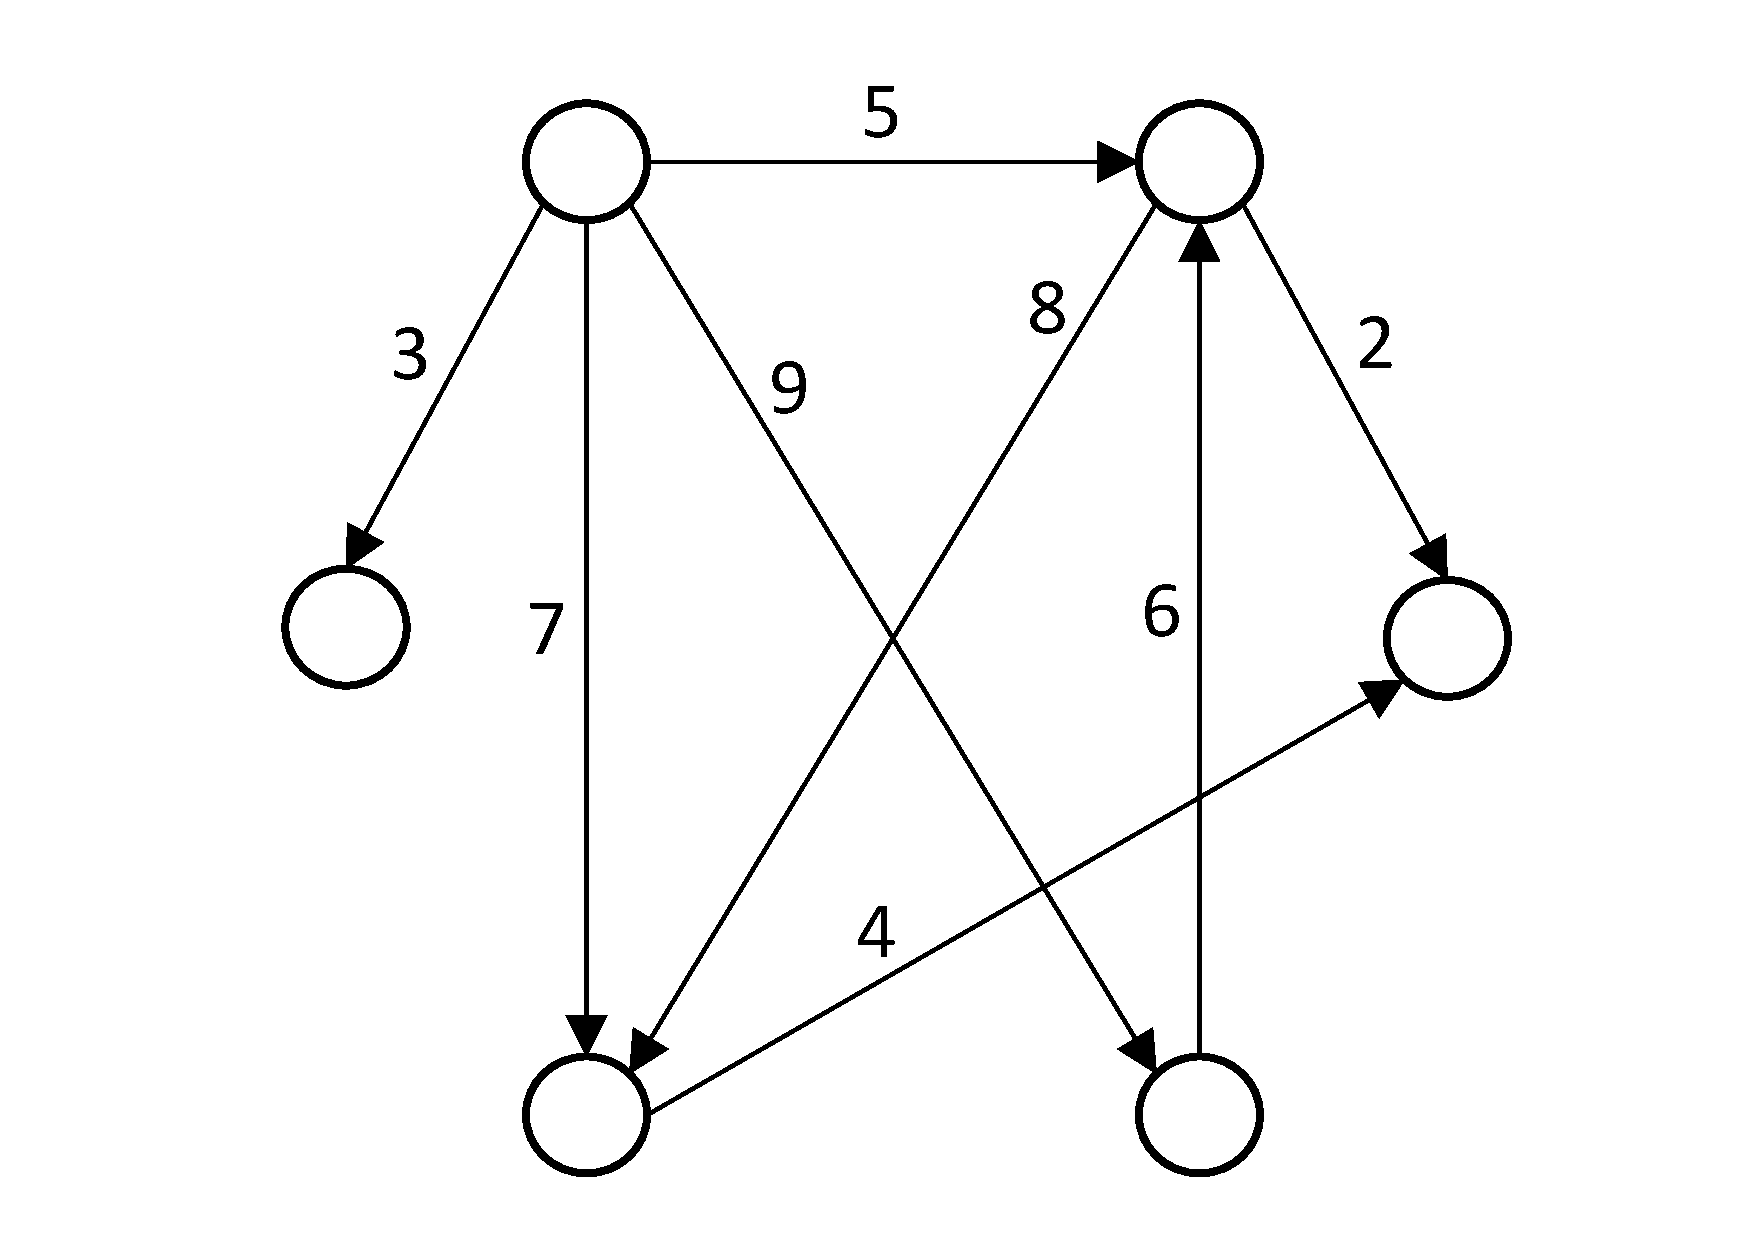
\includegraphics[width=0.3\columnwidth]{chapter2Fig/有向有权重.pdf}}\hfil
	
	\caption{复杂网络图的表示}
	\label{fig2: network} %% label for entire figure
	
\end{figure}

\subsubsection{复杂网络的统计性质}
复杂网络的统计性质主要有:网络的度分布,异质性,同配性,聚类系数,平均最短路径 \cite{汪小帆2006}。

(1) 网络的度分布

对于无向网络而言,一个节点的度,就是节点周围邻居节点的个数。
对于有向网络而言,节点的度分为入度和出度。
特别地,网络的平均度$ <k> $有:
\begin{equation}
<k> = \frac{\sum_{i=1}^{N}{k_i}}{N}.
\end{equation}
其中,$ N $代表网络节点个数,$ k_i $代表节点$ i $的度。

(2) 异质性

网络的异质性描述了节点连接多样性的系数。
网络的异质性越高,代表网络有更多性质不同的节点。
网络的异质性定义为:
\begin{equation}
H = \frac{<k^2>}{<k>^2}.
\end{equation}

(3) 同配性

网络的同配性描述了网络中度相近的节点是否倾向于相互连接的情况。
一般通过皮尔森系数来计算网络的同配系数:
\begin{equation}
r = \frac{M^{-1}\sum_{i}{j_ik_i}-[M^{-1}\sum_{i}\frac{1}{2}{(j_i+k_i)}]^2}{M^{-1}\sum_{i}\frac{1}{2}{(j_i^2+k_i^2)}-[M^{-1}\sum_{i}{\frac{1}{2}(j_i+k_i)}]^2}.
\end{equation}
其中,$ j_i $和$ k_i $分别为第$ i $条边所连节点的度,$ M $为网络边的总数。
若$ r>0 $,代表该网络是同配的,网络中的节点更倾向于连接与之度相近的节点;
若$ r<0 $,代表该网络是异配的,网络中度较大的节点更倾向于连接那些度较小的节点。

(4) 聚类系数

所谓“物以类聚”,我朋友的朋友大概率还是我的朋友,网络的聚类系数描述了这种可能性。
一般而言,网络聚类系数分类为:局部聚类系数和整体聚类系数。在无向图中,单个节点聚类系数定义为:
\begin{equation}
C(i) = \frac{2|\{e_{jk}:v_j,v_k\in L(i), e_{ij}\in E\}|}{k_i(k_i-1)}.
\end{equation}
其中,$ L(i) $代表与节点$ i $相连的所有节点集合,$ k_i $代表节点的度。
换句话说,节点的局部聚类系数等于与它相连的顶点所连边的数量,除以这些顶点可以连出的最大边数。
特别地,网络的平均聚类系数$ <C> $为该网路中所有节点聚类系数的算数平均数。

(5) 平均最短路径

平均最短路径描述了网络节点间的分离程度,定义为:
\begin{equation}
<d> = \frac{\sum_{i=1}^{N}\sum_{j=1}^{N}d(i,j)}{N^2}.
\end{equation}
其中,$ d(i,j) $指的是节点$ i $和节点$ j $的最短路径长度。

\subsubsection{常见网络的模型}
网络的拓扑结构千变万化,在这里简要介绍常见的三种规则网络模型和三种随机网络模型。

(1) 规则网络模型

常见的规则网络模型有:全局耦合网络、最近邻耦合网络、星形网络。
全局耦合网络也称完全图,如图\ref{Fig2:several_network} (a),指的是网络中任意两个节点都存在连接的边。
很明显,全局耦合网络的连边随着节点数量的增加呈线指数增长曲线。
虽然全局耦合网络任意两个节点之间都可以进行信息交流,但在现实生活中,维护这样一个网络所需要的成本太高。
事实上,很多大型网络都是稀疏的,他们边的数量最多是$ O(N) $。
最近邻耦合网络,如图\ref{Fig2:several_network} (b),指的是网络的节点只与其相邻的节点互连,网络整体成为了一个环状。最近邻耦合网络具有高聚类的特性。
星形网络,如图\ref{Fig2:several_network} (c),只有一个节点与其他所有节点相连,不同节点之间的信息交流极大地依赖于中心节点。电话网络中总机和分机的连接采用的就是星形网络。星形网络稳定性较好,易于扩展,但实际操作过程中布线困难,依赖中心节点。如果中心节点收到毁坏,则网络会陷入瘫痪。

\begin{figure}[ht]
	\centering
	\subfigure[全局耦合网络]{
		%%\label{2DSF_1} %% label for first subfigure
		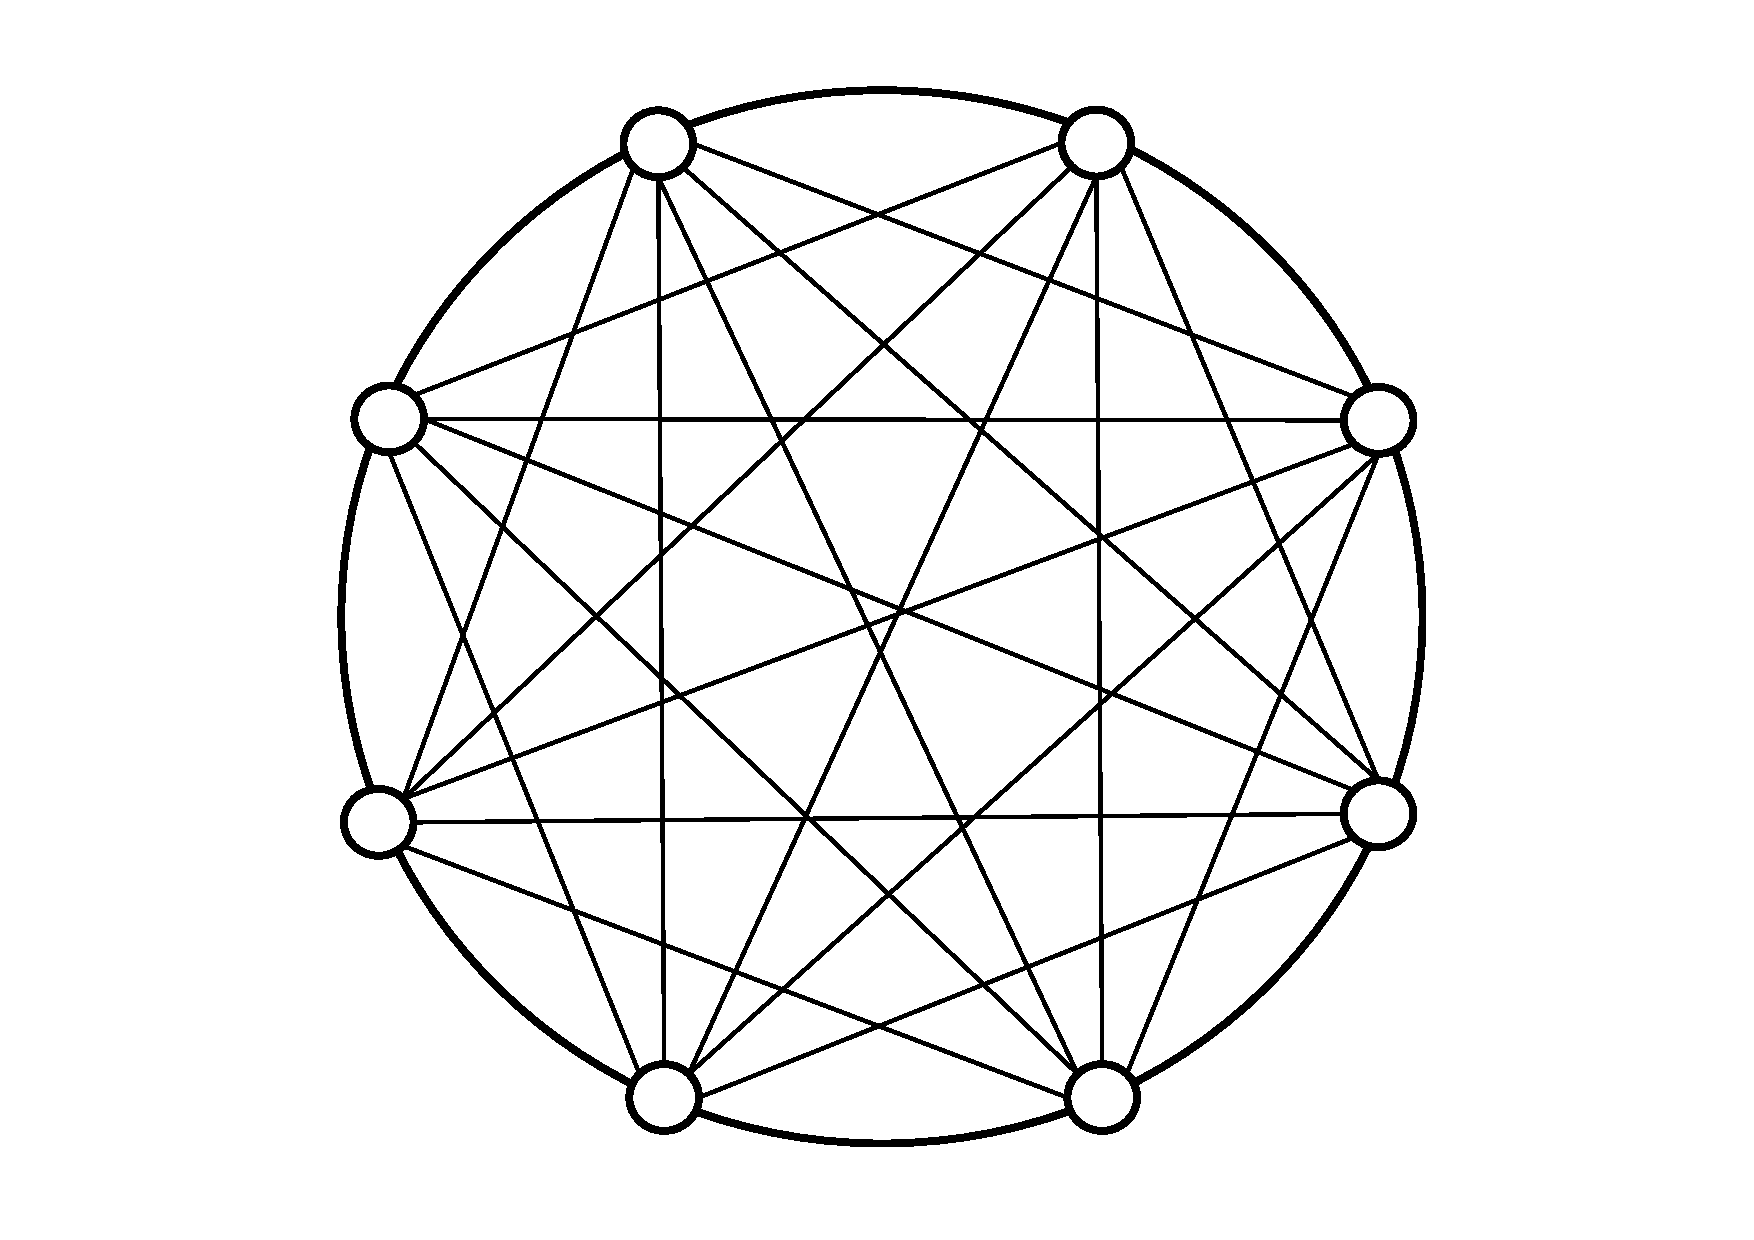
\includegraphics[width=0.3\columnwidth]{chapter2Fig/全局耦合网络.pdf}}\hfil
	\subfigure[最近邻耦合网络]{
		%%\label{2DSF_2} %% label for second subfigure
		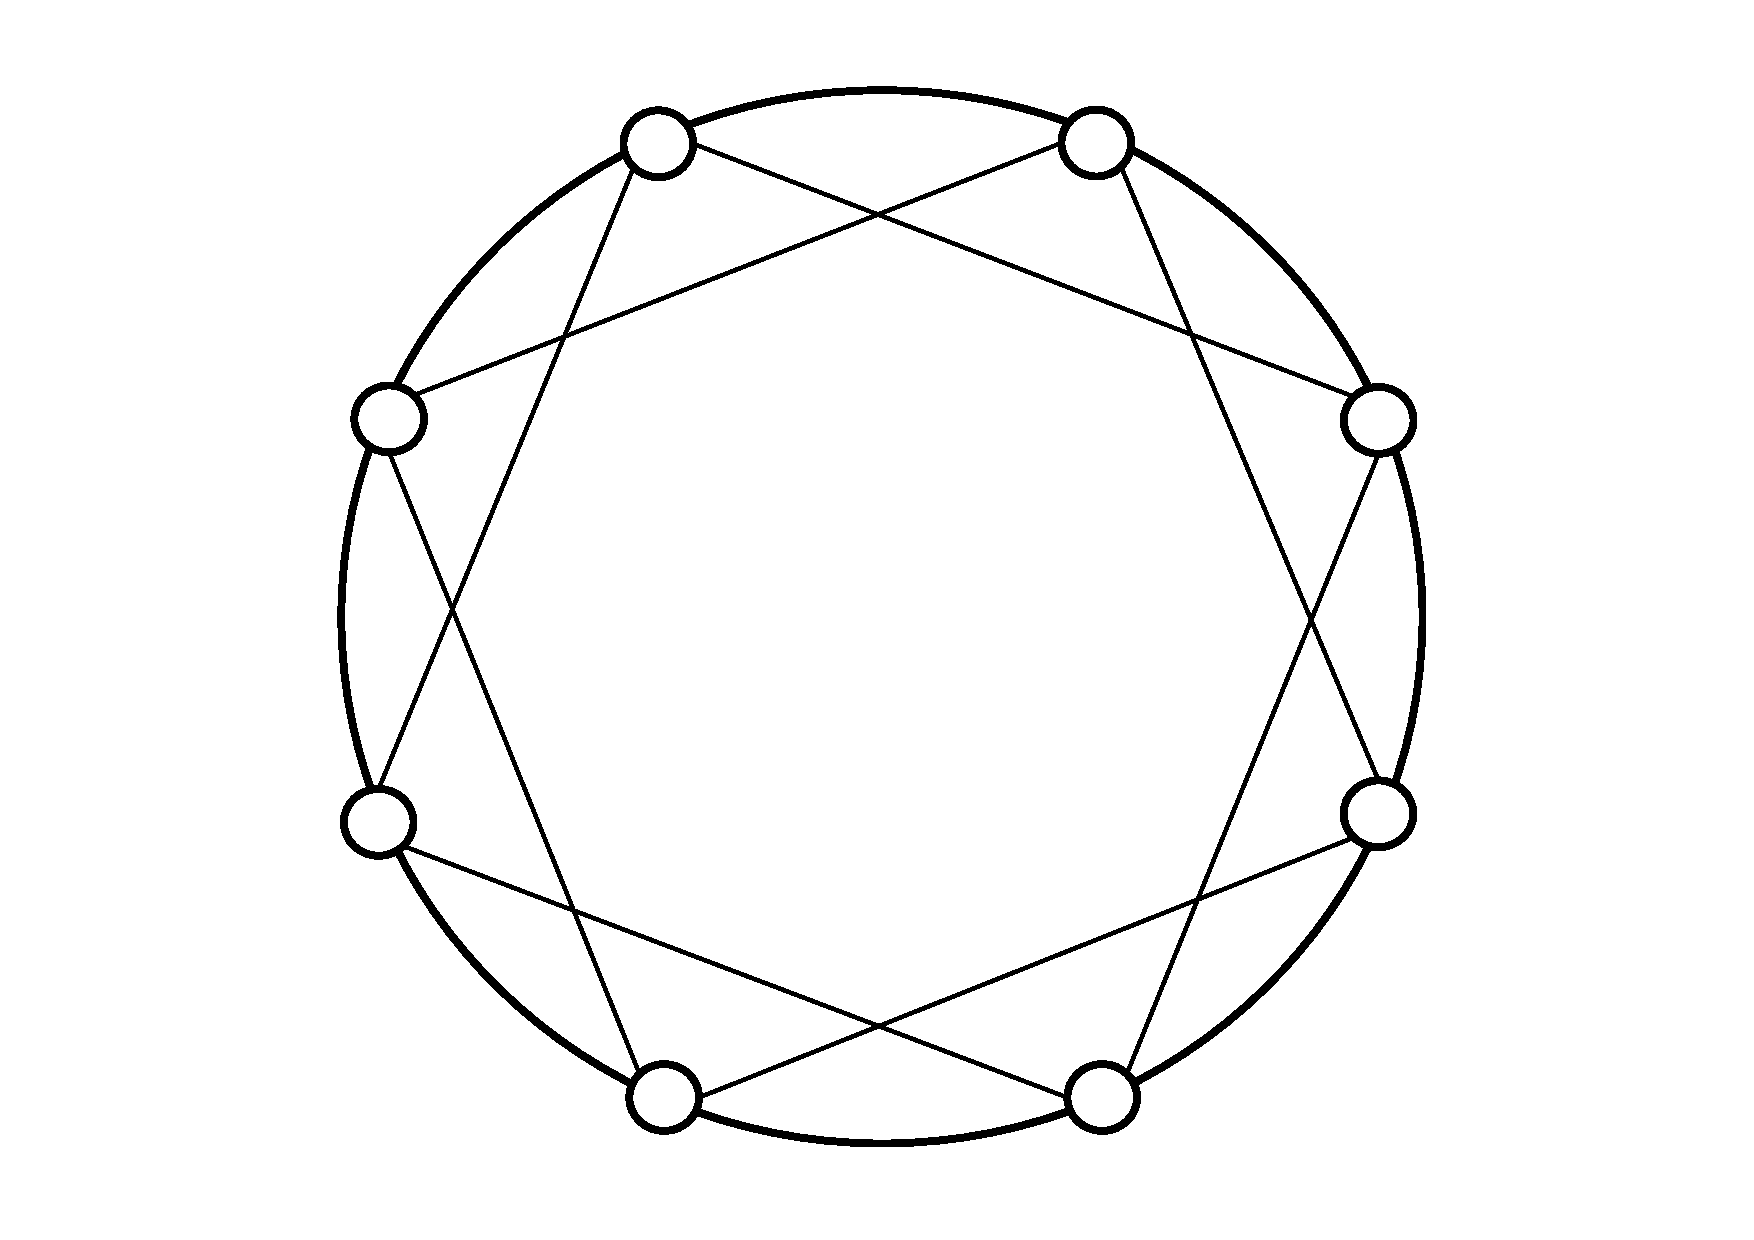
\includegraphics[width=0.3\columnwidth]{chapter2Fig/最近邻耦合网络.pdf}}	
	\subfigure[星形网络]{
		%%\label{2DSF_3} %% label for first subfigure
		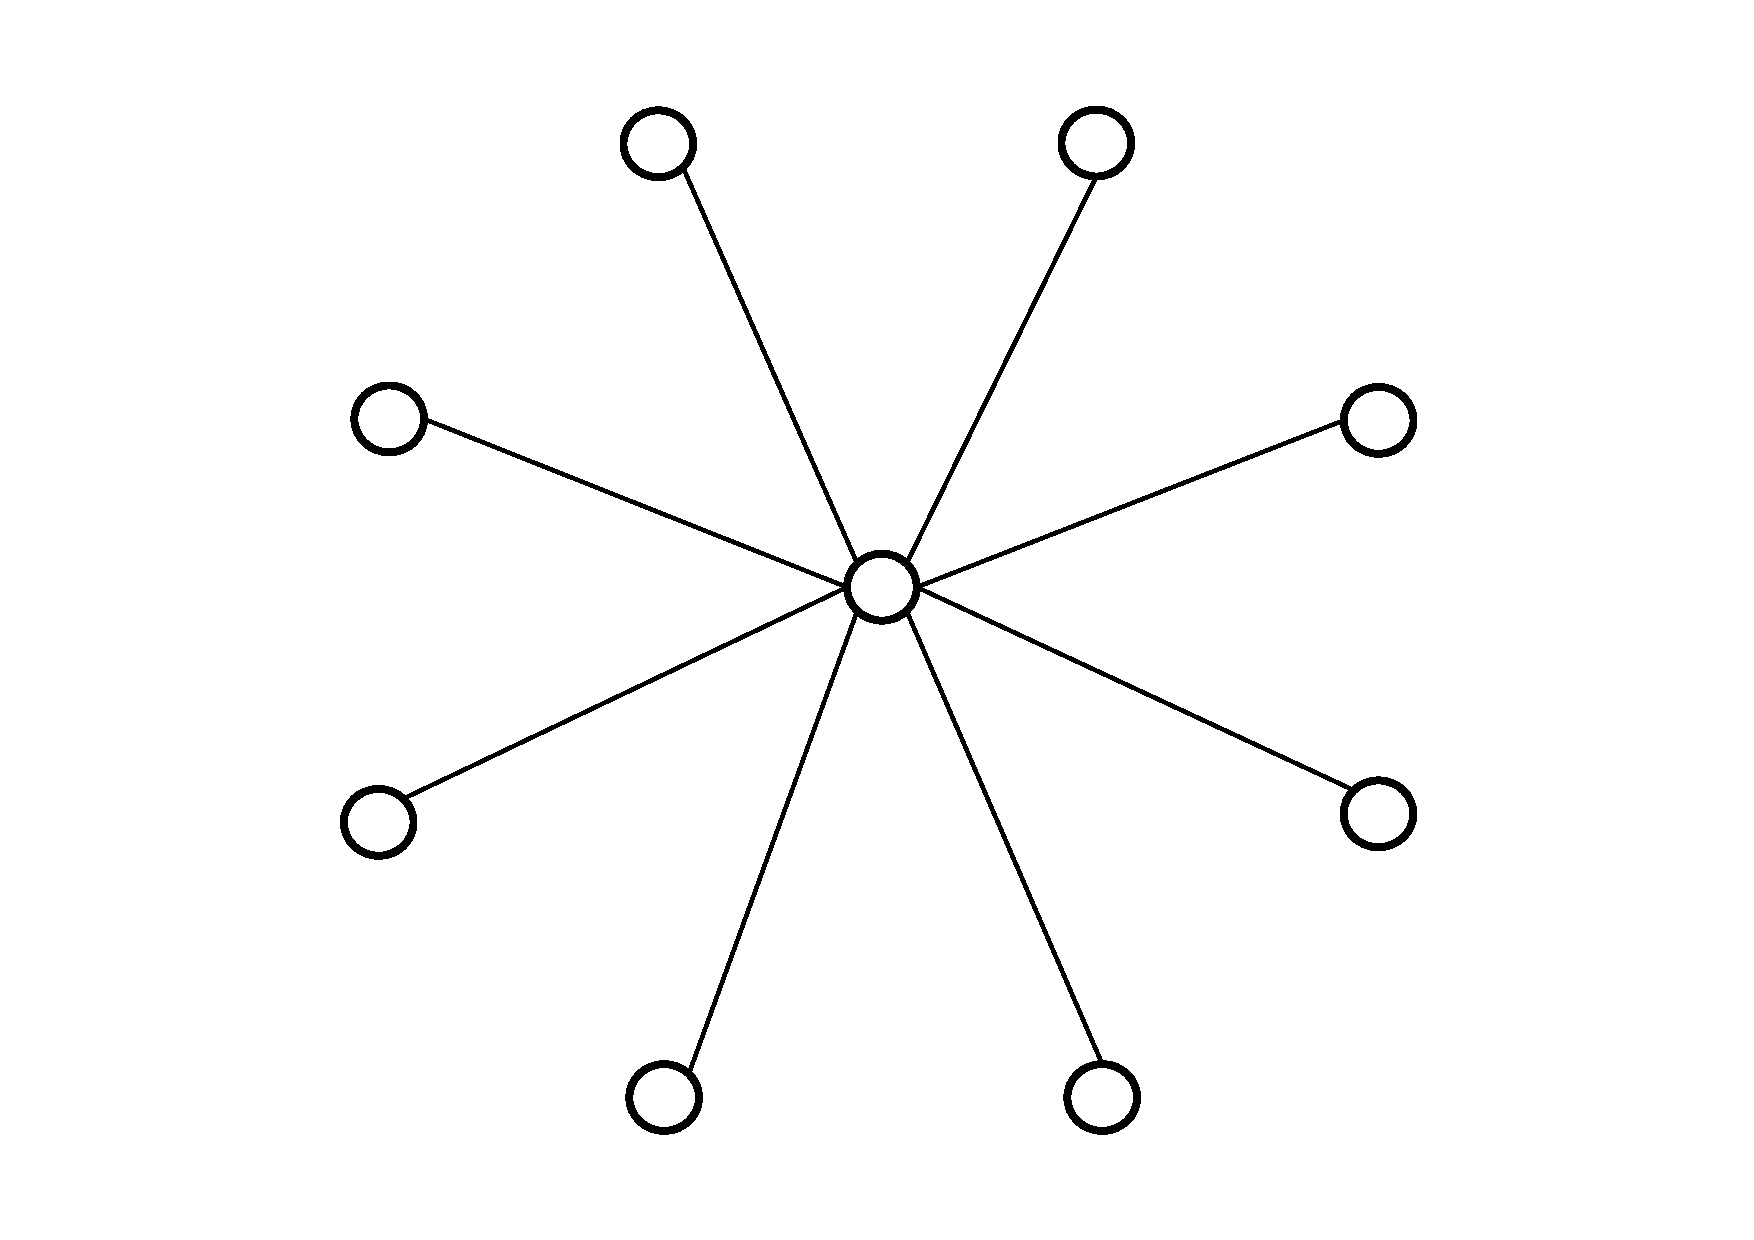
\includegraphics[width=0.3\columnwidth]{chapter2Fig/星形耦合网络.pdf}}\hfil
	
	\caption{几种规则网络}
	\label{Fig2:several_network}
	%\label{figure_2DSF} %% label for entire figure	
\end{figure}




(2) ER(Erd\"{o}s-R{\'e}nyi)随机网络 \cite{Erdoes1959}

ER随机网络又称ER随机图。ER随机图有两种构造方式:
1. $ G(N,p) $,给定$ N $个节点以及节点间的连边概率$ p $,两两节点按照概率$ p $进行连边,直到所有的节点对都被选择;
2. $ G(N,M) $,给定$ N $个节点以及需要添加的边数$ M $,随机选择一组没有进行连边的节点,在他们之间连边,直到所有边数$ M $已被添加完。
如图\ref{Fig: random} (a),该ER随机网络由$ 50 $个节点,节点间连边概率为$ 0.1 $构造而成。

\begin{figure}[t]
	\centering
	\subfigure[ER随机网络]{
		%%\label{2DSF_1} %% label for first subfigure
		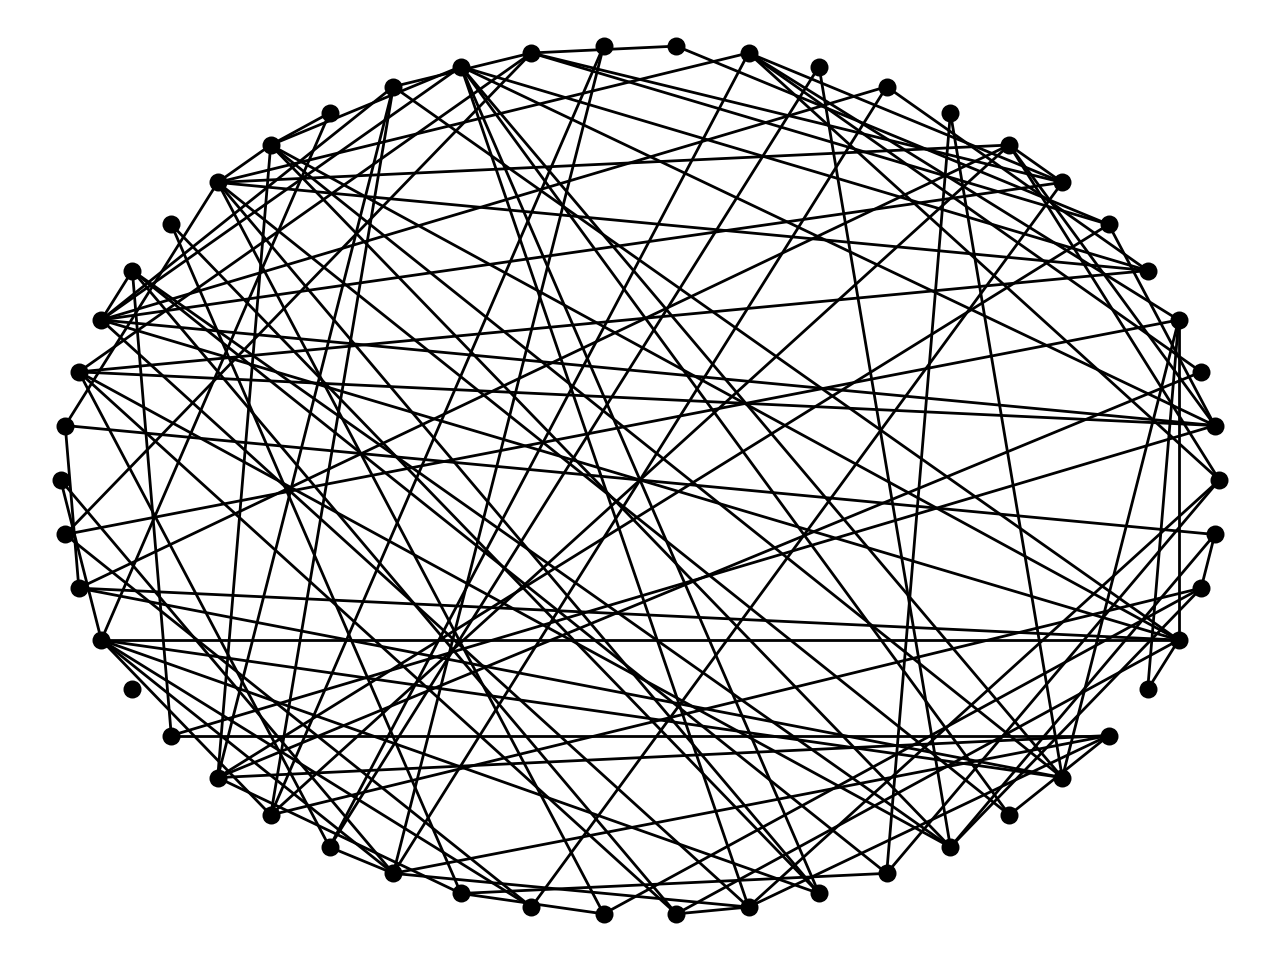
\includegraphics[width=0.3\columnwidth]{chapter2Fig/ER.png}}\hfil
	\subfigure[WS小世界网络]{
		%%\label{2DSF_2} %% label for second subfigure
		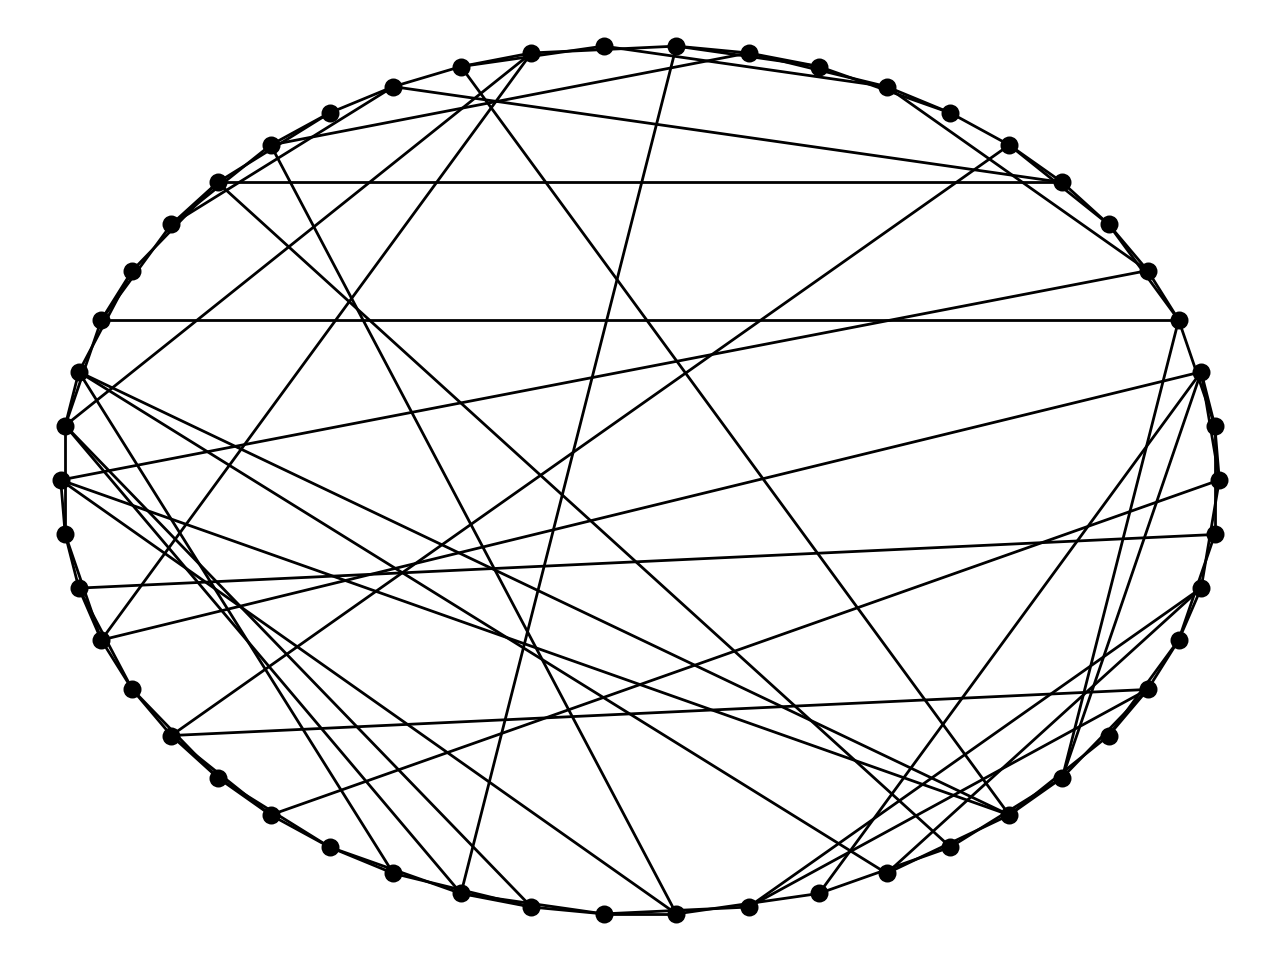
\includegraphics[width=0.3\columnwidth]{chapter2Fig/WS.png}}	
	\subfigure[BA无标度网络]{
		%%\label{2DSF_3} %% label for first subfigure
		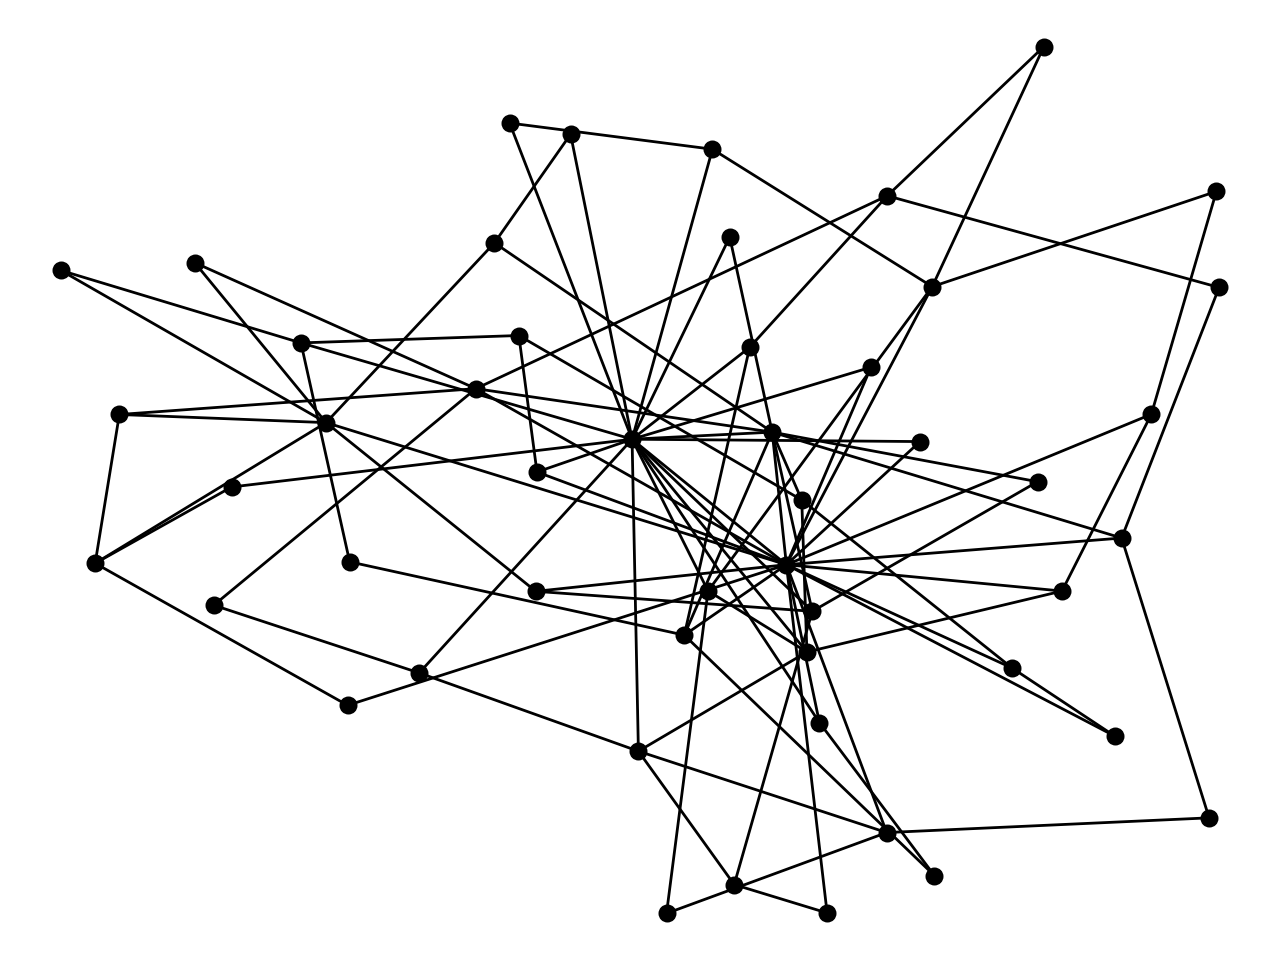
\includegraphics[width=0.3\columnwidth]{chapter2Fig/BA.png}}\hfil
	
	\caption{几种随机网络}
	\label{Fig: random}
	%\label{figure_2DSF} %% label for entire figure	
\end{figure}

(3) WS (Watts和Strogatz) 小世界网络 \cite{Watts1998}

现实中的网络通常具有小世界现象,即:虽然网络中有些节点不具有连边,但任意两个节点之间的最短路径长度远小于节点的数量。
“六度分隔理论”就是对小世界现象的最好阐述,“六度分隔理论”是指,人与陌生人的关系不超过六重,你通过六个人就能够认识世界上任何人。
由于ER随机图无法描述这种小世界这种特性,Watts和Strogatz提出了WS小世界模型算法:
1. 初始网络是有$ N $个节点的最近邻耦合网络,每个节点都和与之左右相邻的$ K/2 $个节点直接相连,$ K $是偶数;
2. 以概率$ p $随机重连初始网络的原有边,重连方式为边的一个节点不变,另一个节点随机选择,且规定在无重边和自环。
如图\ref{Fig: random} (b),该WS小世界网络有$ 50 $个节点,每个节点有$ 4 $个邻居,以概率$ 0.3 $进行重连边。


(4) BA (Barab\'{a}si和Albert) 无标度网络 \cite{Durrett2007}

Barab\'{a}si和Albert发现,在现实生活中,很多网络不同于ER随机图的完全随机,它们的度都近似服从于泊松分布,例如:WWW网络、蛋白质网络、Internet网络等等。
这类网络的度分布在平均值附近有一个峰值,然后服从指数迅速衰减。
于是,他们提出了实际网络中出现的重要特性:
1. 网络的增长。在现实网络中,网络的规模是不断增长的,具体表现为节点数量的增加。例如,在人际关系网络中,人们每天都在认识新的人;
2. 优先连接。网络的规模在扩大的同时,新增的节点更倾向于连接那些已有的高连接度的节点。例如在论文引文网络中,新发表的文章更倾向于引用那些已经被广泛引用的文献。

基于这两个特性,Barab\'{a}si和Albert提出了BA无标度网络算法:
1. 初始网络是一个全局耦合网络,有$ m_0 $个节点,以后每加入一个新节点,则新节点连接$ m $条边到已存在的节点上,且满足$ m<m_0 $;
2. 新节点与已存在节点$ i $连边的概率是:$ \Pi_i={k_i}/ {\sum_{j}{k_j}} $,其中,$ j $为已存在的网络节点,直至节点数量满足要求。
如图\ref{Fig: random} (c),该BA无标度网络有$ 50 $个节点,每次随机加入$ 2 $条连边。

\subsection{同步和控制模型}
网络的控制问题从同步问题而来,而同步问题中最经典的就是Kuramoto相位同步模型。因此,本节从经典的相位同步出发,简单讲解了相位同步,然后关联到一般性的同步过程和网络牵制控制过程。

\subsubsection{Kuramoto同步模型}
一般认为,如果两个耦合的节点的相位$ \theta_i $和$ \theta_j $以一定的比率$ m:n $锁定,并小于某个给定的常数$ \epsilon $,即$ |m\theta_i-n\theta_j|<\epsilon $,则称这两个节点达到了相位同步。相位同步是一种简单的同步,在现实生活中很多应用,如发电机之间的并列运行,导航定位等等。相位同步中,最经典的是Kuramoto同步模型,在这个模型中,每个振子(节点)的动力学方程可以描述成 \cite{Rodrigues2016}:

\begin{equation}
\frac{d\theta_i}{dt}=\omega_i+\frac{c}{N}\sum_{j=1}^{N}(\sin \theta_j-\sin \theta_j), \quad i=1,...,N.
\end{equation}
其中,$ \theta_i $和$ \omega_i $代表第$ i $个的振子的相位和固有频率,$ N $代表整个系统共有$ N $个振子,$ c>0 $为节点之间的耦合强度。


从上述的振子的动力学方程中可以看到,每个振子的相位变化不仅和自身的固有频率$ \omega_i $相关,还与其耦合的节点的相位$ \theta_j $有关。一般认为,在全耦合的振子系统中,耦合强度$ c $足够大时,系统中所有的振子会趋近于同步状态。
如图 \ref{Fig: kuramoto} ,在有20个振子的全耦合网络上模拟了振子同步的过程,耦合强度$ c=1 $,振子震动频率为1赫兹,横纵坐标分别取时间和相位的正弦值。从图中可以很明显地发现,在这个系统中,随着时间的增加,振子的相位趋近于一致,即整个系统是相位同步的。

\begin{figure}[ht]%{.5\linewidth}
	\centering
	% Requires \usepackage{graphicx}
	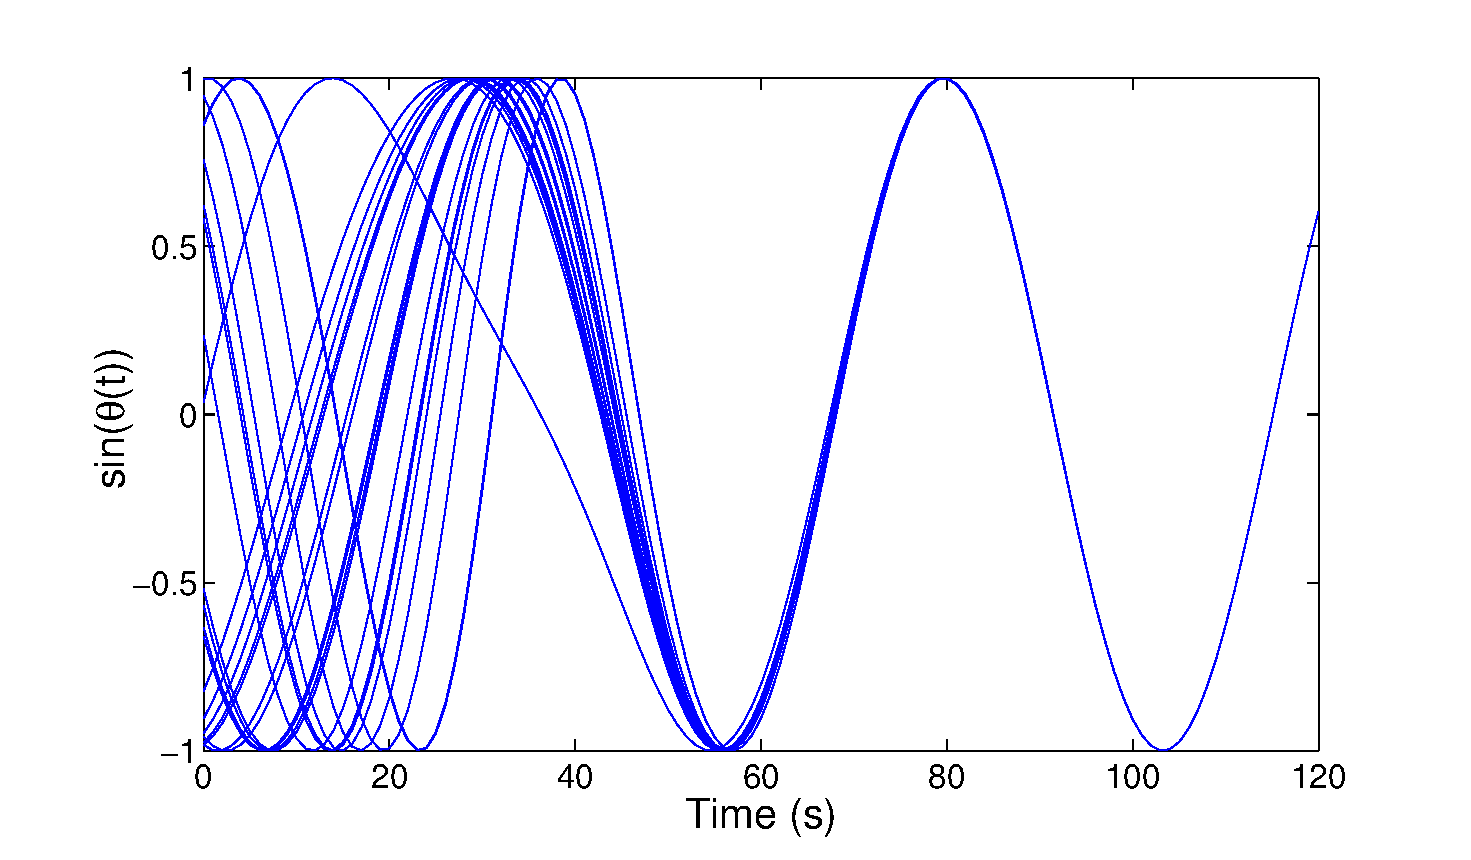
\includegraphics[width=0.9\columnwidth]{chapter2Fig/kuramoto}\\
	% 
	\caption{kuramoto模型振子同步情况}
	\label{Fig: kuramoto}	
	
\end{figure}



\subsubsection{网络同步控制模型}
\label{Sec: control}
现在考虑到一般情况下的同步问题,现给定一个网络$ G = (V, E) $,该网络由$ N=|V| $个节点和$ |E| $条连边构成。
该网络的邻接矩阵可以表示为:$ A=(a_{ij})_{N\times N} $,$a_{ij}=1$ 如果 $(i,j)\in E$,否则$a_{ij}=0$。
那么,该网络的拉普拉斯矩阵有:$ L=(l_{ij})_{N \times N}$,其中, $ l_{ii} $ 为节点$ i $的度,$ l_{ij}=-a_{ij} (i \neq j) $。
另外,网络中每个节点都有状态:$ \textbf{x}_i =(x_{i1},x_{i2},...,x_{in})^T \in R^n, \quad \forall i\in V $。
在连续时间系统中,网络的每个节点的动力学方程可以描述为 \cite{汪小帆2006}:
\begin{equation}
\frac{d\textbf{x}_i}{dt} = f(\textbf{x}_i)-c\sum_{j = 1}^{N}l_{ij}H\textbf{x}_j,\quad \forall i\in V.
\label{Eq: self_dynamics}
\end{equation}

其中,$ f(\textbf{x}_i) $为节点自身的状态改变情况,类似于Kuramoto模型中每个振子的固有频率;$ -c\sum_{j = 1}^{N}l_{ij}H\textbf{x}_j $描述了节点$ i $与其他节点的耦合作用;$ c>0 $ 是耦合强度,描述了节点之间信息交流的强弱;$ H=(h_{ij})_{n \times n} $是一个方阵,描述了节点之间的耦合方式。
和Kuramoto单维的相位同步模型不同,方程\ref{Eq: self_dynamics}描述了网络一般性的同步问题,考虑到了节点$ \textbf{x}_i =(x_{i1},x_{i2},...,x_{in})^T $多个维度的同步情况。

在特殊情况下,网络可能存在自发性同步行为,但在大部分情况下,网络是无法自发性同步的(或同步状态是无法稳定的)。为了使网络达到稳定的同步,可以人为地控制网络中的某些节点,对其施加一个反馈作用。
现记同步稳定状态的平衡点(稳定点):$\overline{\textbf{x}} = (\overline{x}_1, \overline{x}_2, ..., \overline{x}_n)^T$。
为了让网络中的每个节点都达到这种稳定状态,即$x_1(t) = x_2(t) = ... = x_N(t) = \overline{\textbf{x}} $,现对网络的某些节点施加一个反馈作用。假设节点集合$ P $为人为施加的控制节点集合,对于整个网络动力学系统有 \cite{Zhou2019}:
\begin{equation}
\left\{
\begin{aligned}
&\frac{d\textbf{x}_i}{dt} = f(\textbf{x}_i)-c\sum_{j = 1}^{N}l_{ij}H\textbf{x}_j,\quad  i \notin P, \\
&\frac{d\textbf{x}_{i}}{dt} = f(\textbf{x}_{i})-c\sum_{j = 1}^{N}l_{ij}H \textbf{x}_j-cdH(\textbf{x}_{i}-\overline{\textbf{x}}), \quad i\in P.
\end{aligned}
\right.
\label{Eq:all_dynamical}
\end{equation}
其中,$ f(x) $为节点自身状态变化函数,对于稳定点也满足$\frac{d\overline{\textbf{x}}}{dt}=f(\overline{\textbf{x}})$;$ d>0 $代表控制节点的反馈强度。
在网络牵制控制过程中,动力学方程\ref{Eq:all_dynamical}描述了控制节点和普通节点的状态变化过程。从方程可以看到,控制节点通过一个负反馈作用,来调节节点状态加速度的改变,进而引起节点状态的变化;若控制节点的状态大于平衡点($ x_i>\textbf{x}$),则该节点加速度变小,控制节点倾向于“慢下脚步”,等待其他节点;若控制节点的状态小于平衡点($ x_i<\textbf{x} $),则该节点加速度增大,控制节点则“加快脚步”,跟上其他节点的状态。

通过控制节点的负反馈作用,网络也就更容易受到控制,到达同步稳定的状态。然而,最佳控制节点的选择是一个NP-hard问题。因此,为了找到效果最好的牵制控制节点,在本章后续部分,介绍了几种经典的重要节点检测算法。

\subsection{重要节点检测算法}
本节主要介绍了几种经典的重要节点检测算法,包括:度中心性算法,介数中心性算法,接近中心性算法,特征向量中心性算法,PageRank算法,K-shell分解算法和ESI方法。


(1) 度中心性(Degree centrality) \cite{Brodka2011}

以社交网络(微信)为例,一般认为微信好友越多,社交圈子越广,该微信用户也就更为重要,这就是节点度中心性。
无向图的度中心性定义为:
\begin{equation}
DC_i = \frac{k_i}{N-1}.
\end{equation}
很明显,度中心性只与节点的度有关,是网络的一个局部特征。
对于有向图来说,还应考虑到节点的出度和入度。

(2) 介数中心性(Betweenness centrality) \cite{Newman2005}

节点介数中心性指的是节点在其他两个节点最短距离间充当中介的次数。
节点的介数中心性定义为:
\begin{equation}
BC_i = \sum_{i\neq j \neq k}\frac{n_{jk}^i}{g_{jk}}.
\end{equation}
其中,$ g_{jk} $代表节点$ j $和节点$ k $最短路径的条数,$ n_{jk}^i $代表节点$ j $和节点$ k $最短路径经过节点$ i $的次数。
节点的介数中心性越大,代表该节点充当网络中其他节点信息交流的中介次数越多,也就意味着该节点更为重要。

(3) 接近中心性(Closeness centrality) \cite{Okamoto2008}

节点的接近中心性指的是该节点到其他所有节点的最短距离总和的倒数。
无向图的接近中心性定义为:
\begin{equation}
CC_i = \frac{1}{\sum_{j}^{N}d{(i,j)}}.
\end{equation}
其中,$ d(i,j) $指的是节点$ i $到节点$ j $的最短距离。
一般而言,节点接近中心性越高,代表这个节点距离其他节点也越近,节点在空间上也处于比较中间的位置,节点也就更加重要。
对于有向图来说,接近中心性还分为入接近中心性和出接近中心性,分别对应着物理上节点的“整合力”和“辐射力”。

(4) 特征向量中心(eigenvector centrality) \cite{Perra2008}

节点的特征向量中心性认为,某个节点重要性不仅和该节点有关,还与该节点相连的邻居节点有关。
特征向量中心性定义为:
\begin{equation}
EC_i =  c\sum_{j=1}^{N}a_{ij}x_j.
\end{equation}
其中,$ c $是比例常数,$ a_{ij} $代表网络邻接矩阵的元素,$ x_j $代表邻接矩阵和特征值$ c^{-1} $对应的特征向量的元素。

(5) PageRank算法 \cite{Page1999}

谷歌搜索引擎的网页重要性排序采用的就是PageRank算法。
对于网页$ u $而言,该网页的PageRank指标定义为:
\begin{equation}
R(u) = \beta \sum_{v\in B_u}{\frac{R{(v)}}{|B_u|}}.
\end{equation}
其中,$ \beta $是一个归一化常数,$ v $是一个网页,$ B_u $时节点$ u $相邻网页的集合。
对于一个网络来说,节点的PageRank指标越大,也就意味着在随机浏览时,这个节点更大概率被访问到,这个节点也就更加重要。

(6) K-shell分解算法 \cite{Ma1991}

Kitsak等人认为在只有一个传播源的情况下,节点的度和介数并不能精确描述网络节点的传播能力,因而提出了K-shell分解算法。
K-shell分解算法会递归地剥离网络中度数小于或者等于$ k $的节点,
算法流程为:

1)查找网络中所有度为1 $(k = 1) $的节点,将其节点和连边去掉;

2)经过步骤1)后,残余网络中可能会存在度为1的节点;继续重复步骤1),直至网络中不出现度为1的节点,被删除的节点K-shell值定为1;

3)去除度值小于等于2 $ (k<=2) $的节点及其连边,并在残余网络中重复删除操作,被删除的节点K-shell值定为2;

4)依此类推,直至网络上的所有节点都被赋予K-shell值。

该算法实现简单,适用于大型网络,在疾病传播模型中能够很好的找到最有影响力的节点。但在BA无标度网络和树状网络中表现较差,因为在这两个网络中,大部分节点的K-shell值相近,无法区分差异。

(7) ESI方法 \cite{Amani2017}

Amani等人在研究最佳的网络牵制控制节点集合时,提出了一个近似计算节点最大影响力的ESI方法。该方法基于网络拉普拉斯矩阵的谱分析,通过删除节点后观察网络牵制控制传统判据的扰动情况,对节点的脆弱性进行排序。对于一个节点$ i $ 而言,其ESI指数为:
\begin{equation}
ESI(i) = (X_N^i)^2.
\end{equation}
其中,$ X_N $代表了网络拉普拉斯矩阵最大特征值相对应的特征向量,$ X_N^2 $代表特征向量$ X_N $的第$ i $个元素。


\subsection{评价指标}
在本节中,介绍了两个评价指标:节点重叠指数和皮尔森系数。
在第三章和第四章中,节点重叠指数用来比较控制节点之间的差异;在第四章中,皮尔森系数用来比较传统判据和耦合强度范围的相关性。

(1)节点重叠指数HDI(hub depressed index)\cite{Lue2011}

节点重叠指数衡量了节点集合的重叠比例,对于节点集合$ S_1 $与$ S_2 $,节点重叠指数定义为:
\begin{equation}
{\rm HDI}_{S_1\sim S_2} = \frac{|S_1 \cap S_2|}{max(|S_1|,|S_2|)}.
\end{equation}
明显,$ {\rm HDI}_{S_1\sim S_2}\in [0,1] $。$ {\rm HDI}_{S_1 \sim S_2}\rightarrow 0 $代表集合$ S_1 $与$ S_2 $重叠节点越少;$ {\rm HDI}_{S_1\sim S_2}\rightarrow 1 $代表集合重叠节点越多。

(2)皮尔森系数 \cite{LeeRodgers1988}

皮尔森系数衡量了两个变量的相关性,对于变量$ X $与$ Y $,其皮尔森系数定义为:
\begin{equation}
r_{x,y} = \frac{cov(X,Y)}{\rho_X \rho_Y} = \frac{E[(X-E(X))(Y-E(Y)]}{\rho_X \rho_Y}.
\end{equation}
其中,$ cov(X,Y) $代表了变量$ X $与$ Y $的协方差,$ \rho_X $与$ \rho_Y $代表了变量的标准差,$ E(X) $与$ E(Y) $代表了变量$ X $与$ Y $的期望。
此外,$ r_{x,y}\in[-1,1] $。$ r_{x,y}\rightarrow1 $代表变量$ X $与$ Y $趋近于正相关关系;$ r_{x,y}\rightarrow-1 $代表变量$ X $与$ Y $趋近于负相关关系。


\subsection{本章小结}

本章主要介绍了网络科学基础理论,涵盖了复杂网络的主要性质、网络的同步和控制模型、重要节点检测算法等三大内容。


\clearpage
